\subsection{Experimental Setup}
In order to investigate oscillations in twisted string actuators, we have manufactured the testbed shown in Fig.
\ref{fig:ex_setup}. It is comprised of a EC motor (Maxon EC-4pole 22 120W, 18V) equipped with a quadrature optical incremental encoder (1024 CPT), a linear encoder with the resolution of 18 $\mu$m (Avago H9740-1 360 LPI) 
to measure the actual string contraction and a digital controller (32 bit Arm Cortex-M7 216 MHz core-based) 
connected to the motor driver (ESCON 70/10). We have installed a pair of 0.75-mm Dyneema strings in the TSA with the length of 170 mm, just like the ones used in simulation. 

	\begin{figure}
		\centering
		\vspace*{-1mm} 
		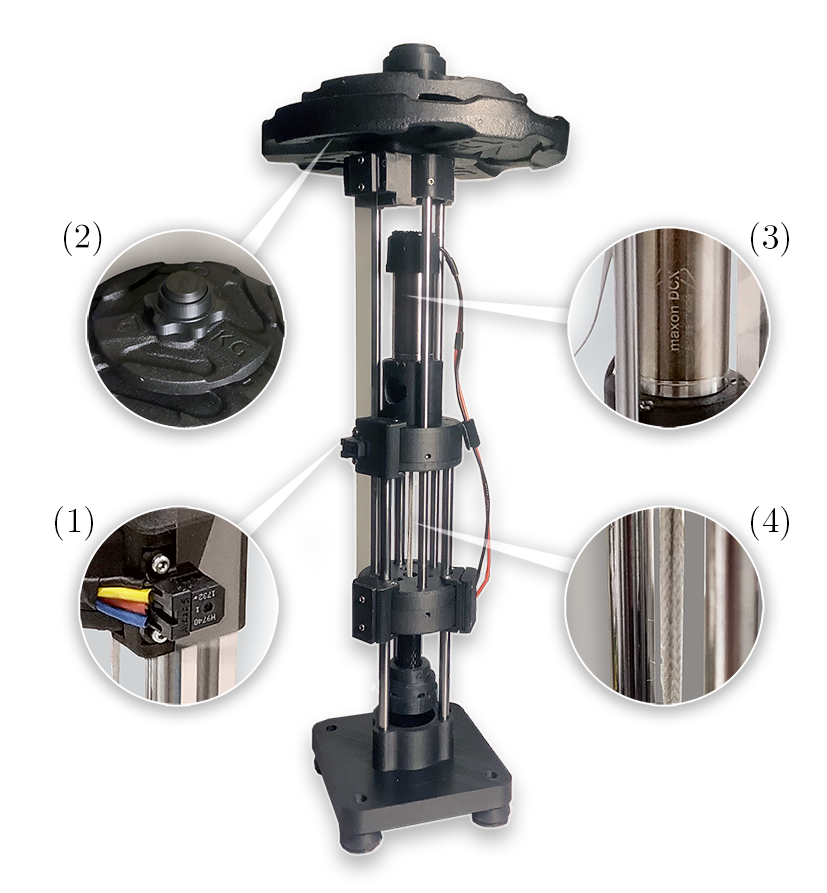
\includegraphics[trim= 0.0cm 0.5cm 0.0cm 0.0cm, width=0.8\columnwidth]{pics/linear_setup.png}
		\caption{Photo of the experimental setup:  1) linear encoder, 2) static payload, 3) EC motor with angular incremental encoder, 4) twisted strings  }
		\label{fig:ex_setup}
		\vspace*{-4mm} 
	\end{figure}

The setup operates as follows. The motor twists the strings, causing their contraction. The strings pull up the bottom mount which moves along three vertical sliders (fixed between the base and the motor mount) and has a optical strip attached to it. Rigidly fixed to the moving mount are three more thin metal rods that support the top platform with a payload. The motion of the optical strip is registered by a stationary optical encoder located at the motor mount.

\subsection{Energy and Phase Trajectories}
After we confirmed the presence of oscillations in a practical setup similar to those suggested by the simulations, our first aim was to try recreate the oscillatory energy behavior presented in Fig. \ref{fig:energies_simulation}. The corresponding experimental plot of major energy components in TSA is given in Fig. \ref{fig:energies_exp}. One can note the similarities between the simulated and experimental energy curves, with the main difference being a slightly lopsided shape of the actuator kinetic energy $E_K^\theta$. This is most likely caused by some effects at play in a practical setup which are not reflected by the simplified energy model, namely, dry friction and unilateral string stiffness (jamming) described in our previous work \cite{nedelchev2020accurate}. However, the general nature of the oscillations, as well as their frequency, was predicted by the simulated results fairly well.
\begin{figure}
		\centering
		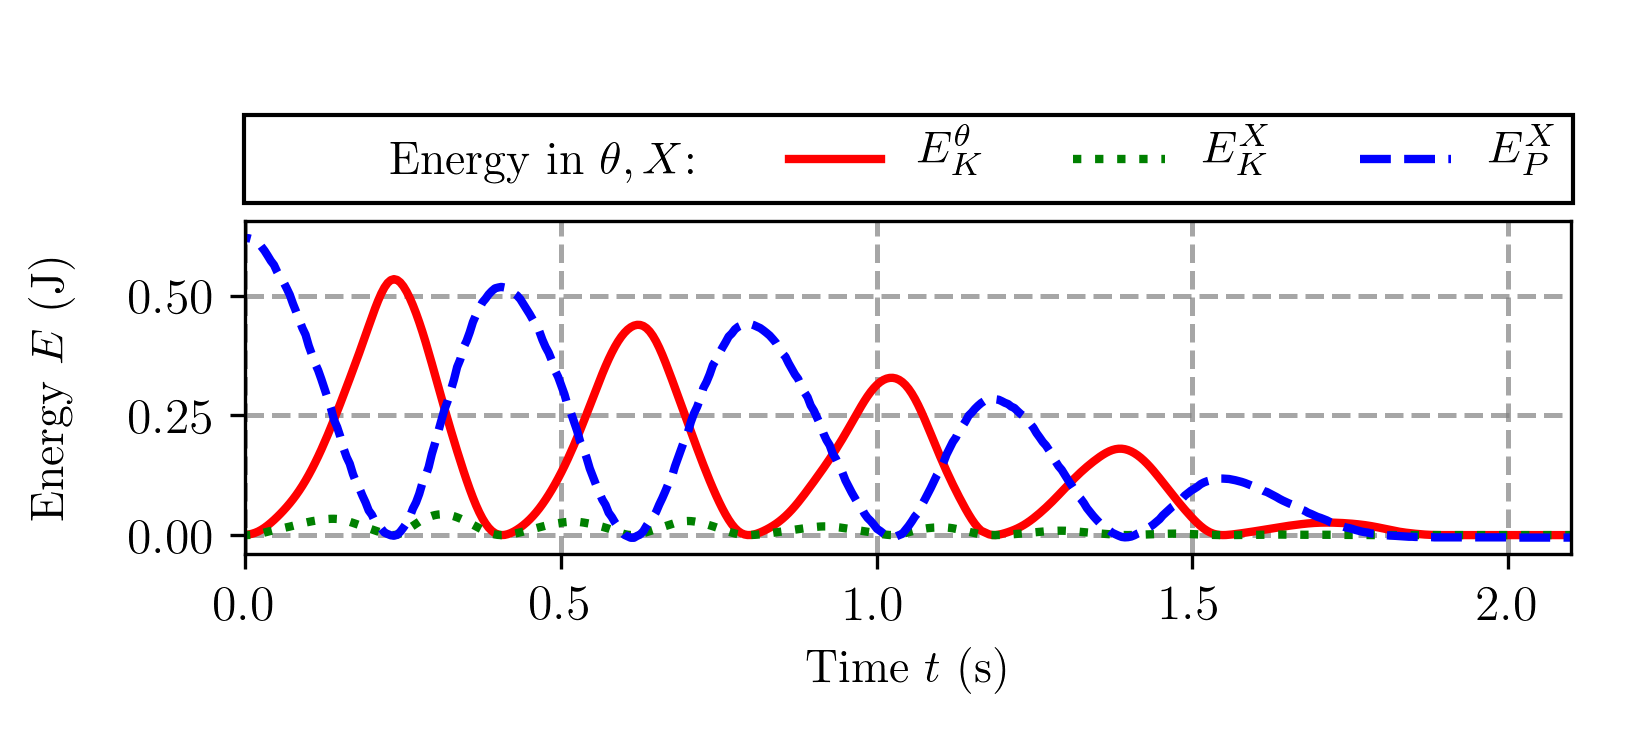
\includegraphics[trim= 0.0cm 1.0cm 0.0cm 0.0cm,width=1.0\columnwidth]{pics/plots/exp_energy_damp.png}
		\caption{Experimental time plots of energy components in a TSA during free oscillations with 90\% of friction compensated for by controller}
 		\label{fig:energies_exp}
		\vspace*{-2mm} 
\end{figure}

Corresponding phase plots in actuator and payload coordinates are presented in Fig. \ref{fig:phase_plots_exp}. Here, the shape difference between simulated and experimental phase trajectories are more apparent, which calls for a deeper analysis if one desires to predict the curves with higher accuracy. However, in this preliminary research we were mainly interested in whether we would be able to predict the peak values of positions and velocities (and the corresponding energy levels) with enough accuracy, and the simplified energy model allows to achieve this. 

\begin{figure}
		\centering
		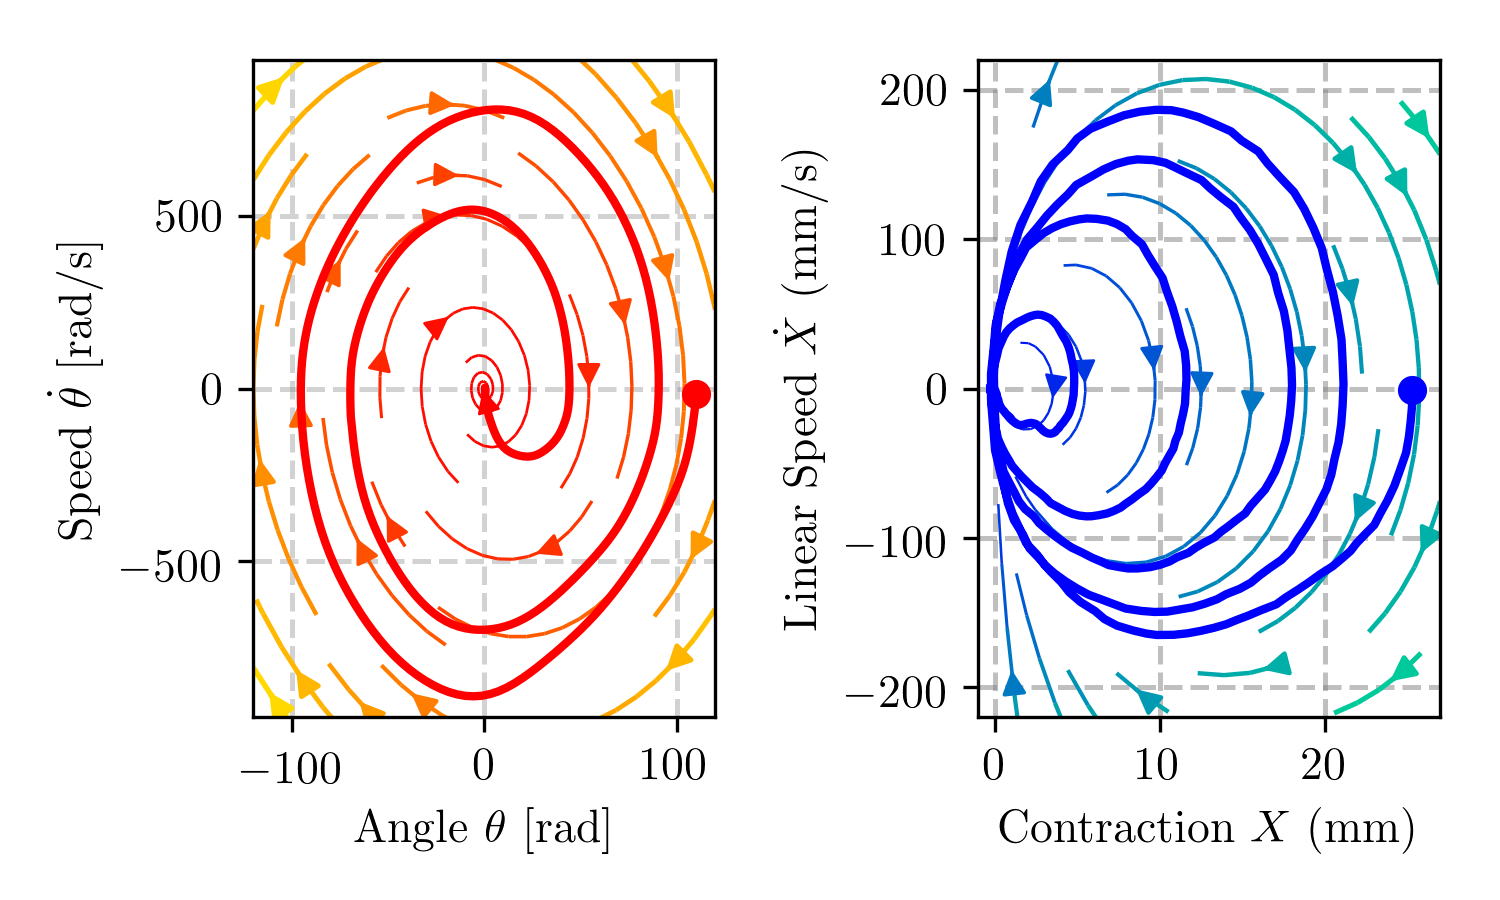
\includegraphics[trim= 0.0cm 1.0cm 0.0cm 0.0cm,width=1.0\columnwidth]{pics/plots/phase_space_experiment.png}
		\vspace*{-2mm} 
		\caption{Experimental phase plots of free oscillations, with the vector fields plotted with help of the proposed model}
 		\label{fig:phase_plots_exp}
\end{figure}

\subsection{Friction Compensation}
Once one has a satisfactory model of free oscillatory response in a twisted string actuator that is confirmed by experiments, one research question that can be asked is how can we use this knowledge to design an energy-efficient controller for TSAs. Since the main causes of power dissipation in the system are the frictional forces, their cancellation (or at least compensation for) would naturally prolong free oscillatory response in the actuator. Thus, we have designed a feedforward control system which would introduce the torque $u = \hat{b}\dot{\theta}$, with a positive term $\hat{b}$ representing our guess of viscous friction coefficient. 

A time plot of three curves, corresponding to damped oscillatory response of TSA for 3 different values of $\hat{b}$ are shown in Fig. \ref{fig:friction_cancellation}. One can note how increased friction compensation leads to prolonged   oscillations, as expected. Thus, if one can fully compensate for friction (e.g. with feedforward/feedback linearization) in a TSA system, it is possible to induce undamped oscillatory response in it with the `natural' frequency. Just like in any undamped system, total energy will remain constant during free oscillations, with kinetic energy of the actuator converted into kinetic and potential energy of the payload, and vice versa. The reverse is also true - if one preserves constant energy levels within a TSA-based system by means of control, they can induce undamped oscillations with minimal control effort, which can be leveraged, for example, when designing a legged robot. 

Energy preservation in TSA is studied in detail in the following section.
\begin{figure}
		\centering
		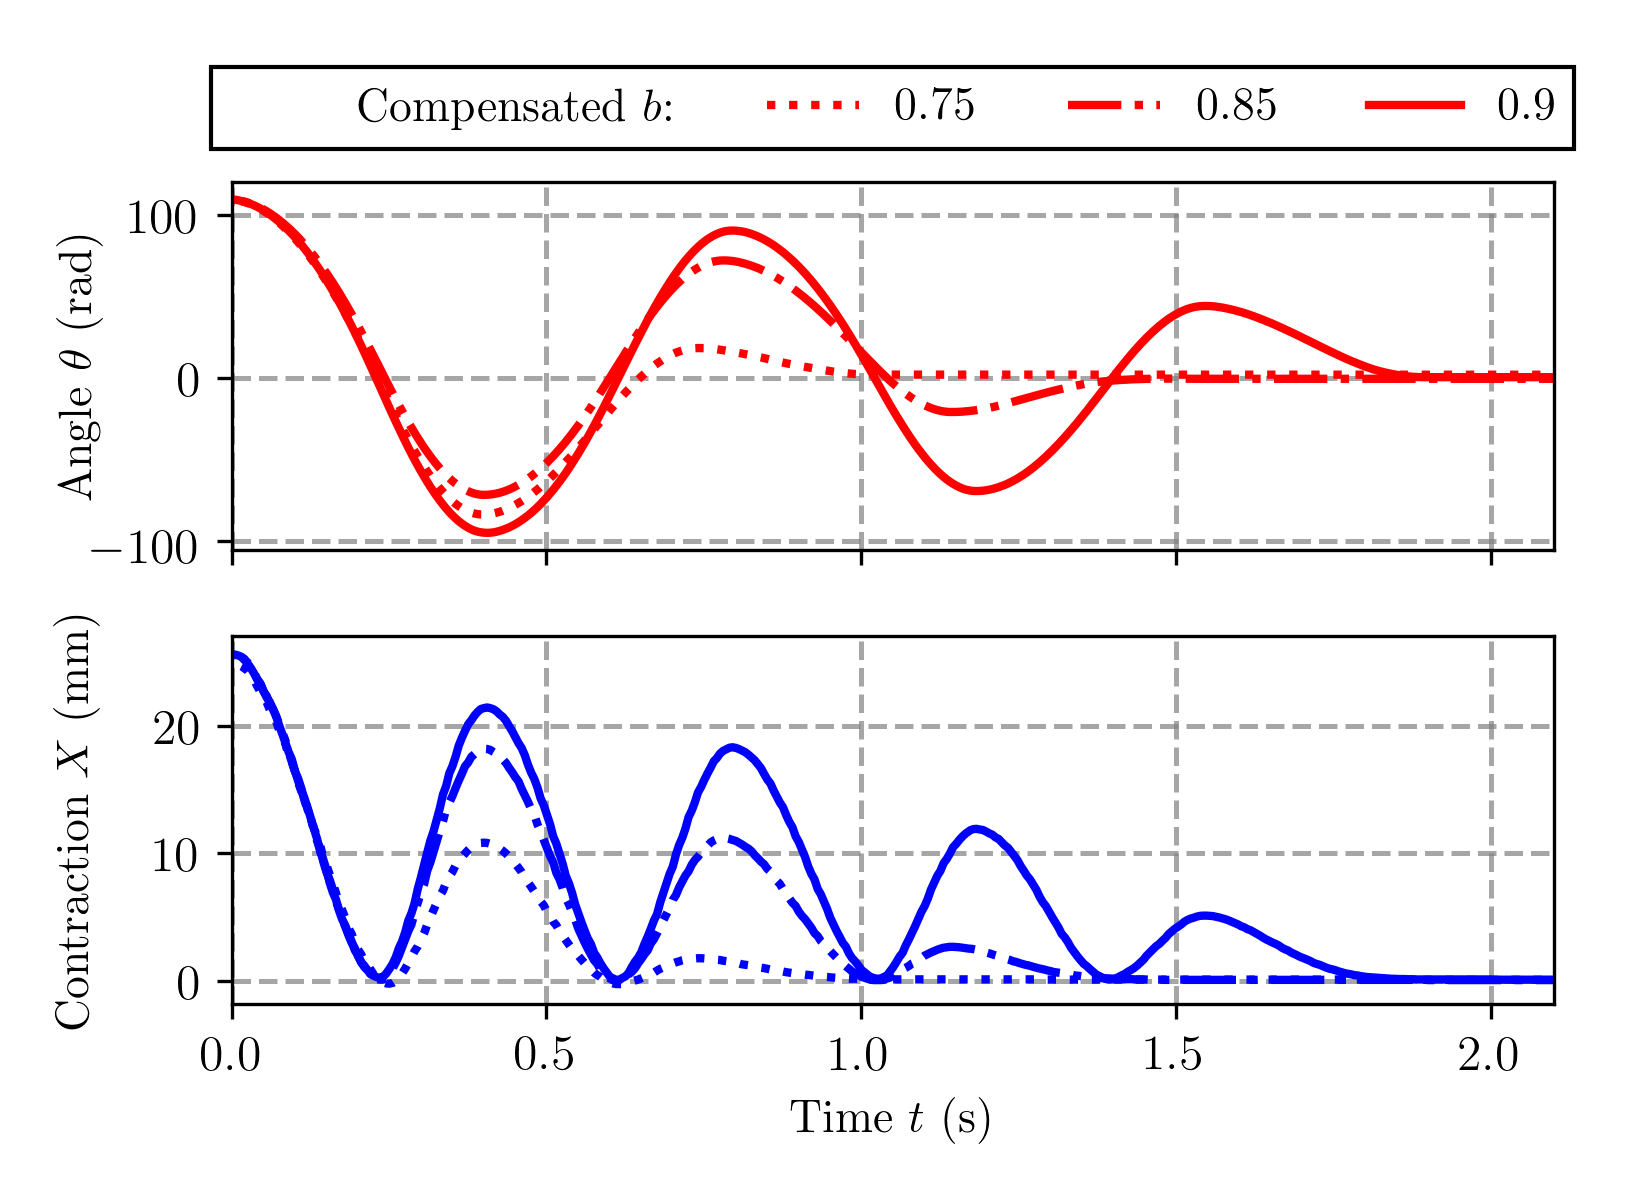
\includegraphics[trim= 0.0cm 1.0cm 0.0cm 0.0cm,width=1.0\columnwidth]{pics/plots/exp_var_damp.png}
		\caption{Time plots of motor angle (top) and payload (bottom) for various levels of friction compensation}
 		\label{fig:friction_cancellation}
		\vspace*{-2mm} 
\end{figure}

